\chapter{Phase Diagrams and Theory Deliverables}
\label{ch:phase-diagrams-theory-deliverables}

\textit{A theory result is not a single successful simulation. It is a map: which mechanisms occur in which parameter regimes, what changes when the network is scaled, and which measurements distinguish asynchronous activity, bistability, metastability, and deterministic irregular dynamics.}

% ============================================================
\section{What Parameters to Sweep}
\label{sec:what-parameters-to-sweep}
% ============================================================

A parameter sweep should be organized around mechanisms rather than around every available constant. For clustered spiking networks, the primary control vector is
%
\begin{equation}
  \theta
  =
  \left(
  g_{EE},
  g_{EI},
  g_{IE},
  g_{II},
  n_E,
  n_I,
  Q,
  \sigma_{\mathrm{fs}},
  \sigma_{\mathrm{quenched}},
  h
  \right),
  \label{eq:phase-diagram-parameter-vector}
\end{equation}
%
where the $g$ parameters control structured coupling, $n_E,n_I$ control cluster sizes, $Q$ controls the number of clusters, $\sigma_{\mathrm{fs}}$ controls finite-size noise, $\sigma_{\mathrm{quenched}}$ controls fixed heterogeneity, and $h$ is external drive or stimulus bias.

Not every sweep should be high-dimensional. Start with two-dimensional slices whose axes have interpretable effects:
%
\begin{equation}
  (g_{EE},h),
  \qquad
  (g_{EE},g_{EI}),
  \qquad
  (g_{EE},n_E),
  \qquad
  (\sigma_{\mathrm{fs}},\sigma_{\mathrm{quenched}}).
  \label{eq:recommended-phase-slices}
\end{equation}
%
Each slice should hold mean input normalization fixed unless the goal is explicitly to study changes in mean input.

For each grid point, save summary statistics rather than only plots: fixed-point count, leading eigenvalue, mean rates, active-cluster occupancy, dwell-time summaries, Fano factors, autocorrelation time, and, for deterministic equations, largest Lyapunov exponent when appropriate.

\begin{figure}[h]
\centering
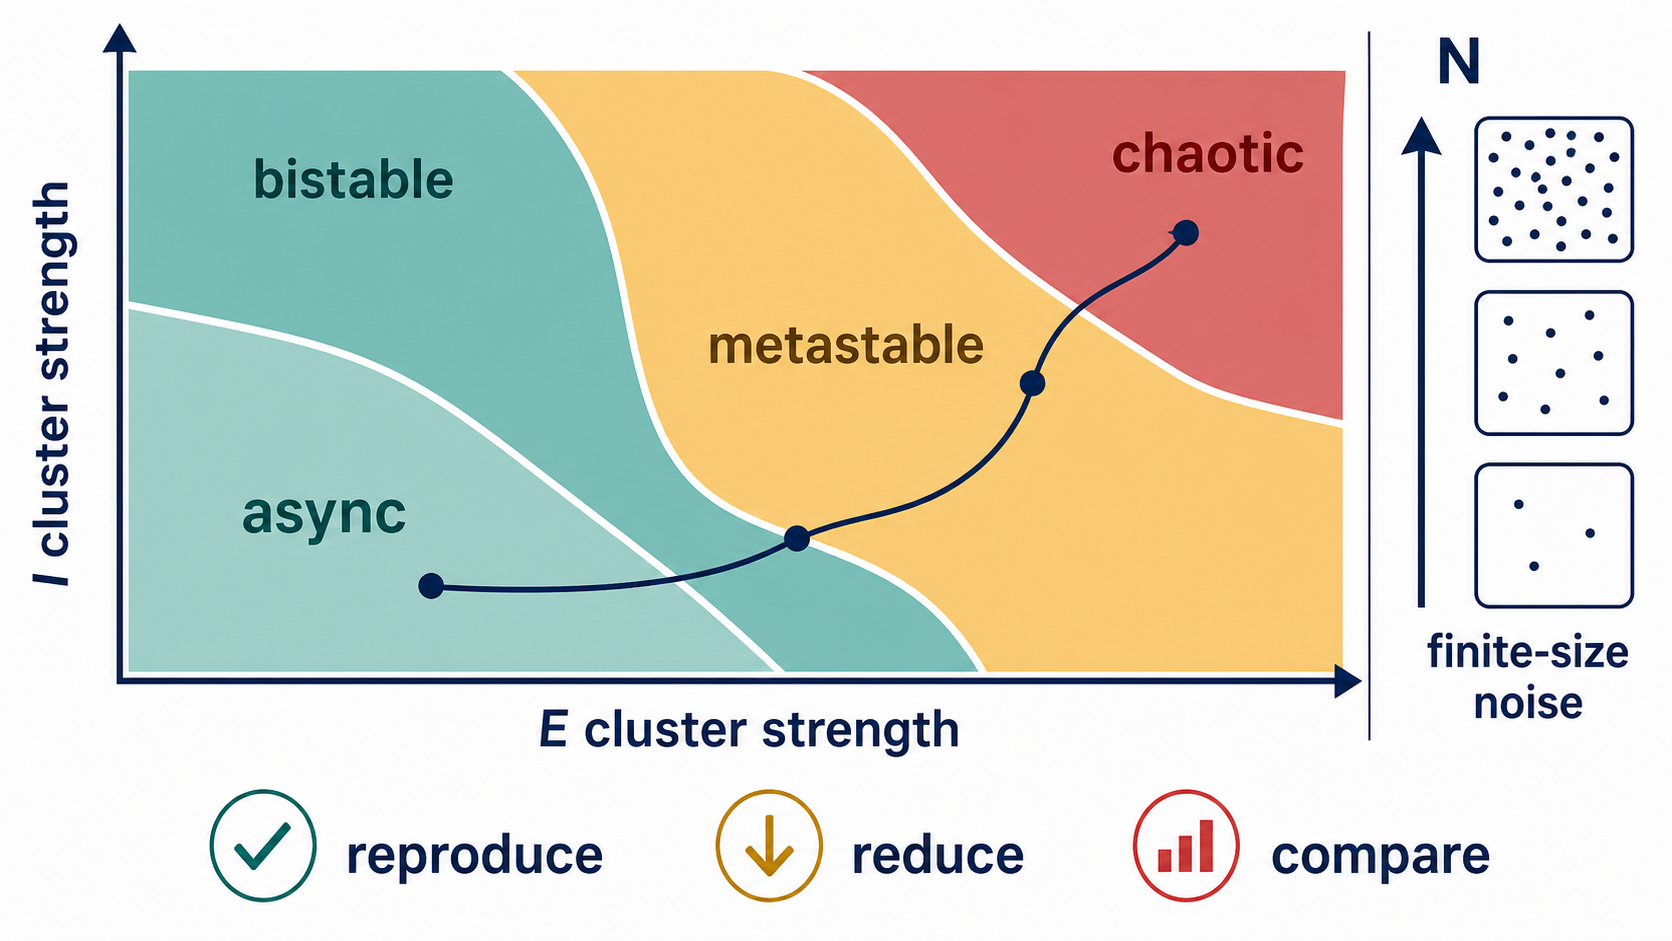
\includegraphics[width=0.95\textwidth]{figures/meso-phase-diagram-roadmap.png}
\caption{A useful theory artifact is a regime map. Sweeping excitatory and inhibitory cluster strength can separate asynchronous, bistable, metastable, and chaotic regions. Repeating the sweep across network size tests whether observed switching is finite-size noise, deterministic mesoscopic structure, or a mixture of both.}
\label{fig:phase-diagram-roadmap}
\end{figure}

% ============================================================
\section{Cluster Strength}
\label{sec:phase-cluster-strength}
% ============================================================

Cluster strength is the first axis because it controls the transition from an unstructured balanced network to a clustered attractor network. A generic definition is
%
\begin{equation}
  g_{EE}
  =
  \frac{W_{+}^{EE}}{W_{0}^{EE}},
  \qquad
  W_{-}^{EE}
  =
  \frac{QW_{0}^{EE}-W_{+}^{EE}}{Q-1},
  \label{eq:cluster-strength-normalization}
\end{equation}
%
for equal cluster sizes. The second equation keeps the mean excitatory coupling fixed.

As $g_{EE}$ increases, the expected sequence is:
%
\begin{enumerate}[leftmargin=*]
  \item weak clustering: asynchronous irregular activity with no distinct up-states;
  \item near bifurcation: slow fluctuations and long autocorrelation, but unreliable state separation;
  \item bistable regime: low and high cluster states coexist;
  \item metastable regime: finite-size noise causes transitions among active-cluster patterns;
  \item pathological regime: runaway, permanent locking, or synchrony if inhibition cannot stabilize recurrent excitation.
\end{enumerate}

The key mathematical diagnostic is the leading stability eigenvalue of a candidate cluster state. If the leading real part approaches zero from below, the state becomes slow and noise-sensitive. If it crosses zero, the deterministic state changes stability.

% ============================================================
\section{Inhibitory-Cluster Strength}
\label{sec:phase-inhibitory-cluster-strength}
% ============================================================

In an E/I-clustered extension, inhibitory structure has several axes. A compact pair is
%
\begin{equation}
  g_{IE}=\frac{W_{+}^{IE}}{W_{0}^{IE}},
  \qquad
  g_{EI}=\frac{W_{+}^{EI}}{W_{0}^{EI}},
  \label{eq:inhibitory-cluster-strengths}
\end{equation}
%
where $g_{IE}$ measures how strongly excitatory clusters recruit their paired inhibitory clusters, and $g_{EI}$ measures how strongly paired inhibitory clusters suppress excitatory clusters.

The product of these pathways enters the fast-inhibition correction:
%
\begin{equation}
  K_{\mathrm{inh}}
  =
  W^{EI}{(\mat{I}+G_I W^{II})}^{-1}G_I W^{IE}.
  \label{eq:inhibitory-correction-strength}
\end{equation}
%
Increasing $g_{IE}$ or $g_{EI}$ strengthens this correction, but the effect depends on inhibitory gain and self-coupling. Stronger local inhibition can stabilize up-states by preventing runaway, or it can destroy up-states by over-cancelling recurrent excitation.

The practical phase diagram should therefore show at least one slice in $(g_{EE},g_{EI})$ or $(g_{IE},g_{EI})$. The expected robust region is a band: enough inhibitory pairing to regularize activity, not so much that attractor states disappear.

% ============================================================
\section{Network Size}
\label{sec:phase-network-size}
% ============================================================

Network size is not a single parameter in clustered networks. The total number of neurons is
%
\begin{equation}
  N = Q(n_E+n_I)
  \label{eq:total-clustered-network-size}
\end{equation}
%
in a paired E/I architecture. Changing $N$ can mean increasing cluster size, increasing the number of clusters, or both.

For the finite-size-driven multistability hypothesis, the cleanest size sweep keeps $Q$ fixed and increases $n_E,n_I$ while preserving deterministic coupling. The finite-size noise term then changes as
%
\begin{equation}
  \sigma_{\mathrm{eff},k}^{a}
  \propto
  \frac{1}{\sqrt{n_a}},
  \qquad
  a\in\{E,I\}.
  \label{eq:size-noise-scaling-ei}
\end{equation}
%
The predicted outcome is reduced within-state variance and longer dwell times.

Increasing $Q$ asks a different question: how many competing attractor labels the model can support. Large $Q$ can create more state combinations, more contrast modes, and more opportunities for deterministic high-dimensional dynamics. Do not mix the two size questions without labeling the scaling protocol.

% ============================================================
\section{Cluster Size}
\label{sec:phase-cluster-size}
% ============================================================

Cluster size is the most direct knob for testing finite-size switching. With fixed cluster count and fixed deterministic parameters, the stochastic mesoscopic model has the form
%
\begin{equation}
  \dd \vec x
  =
  f(\vec x;\theta)\,\dd t
  +
  \frac{1}{\sqrt n}B(\vec x;\theta)\,\dd \vec W_t .
  \label{eq:cluster-size-phase-sde}
\end{equation}
%
The drift $f$ is unchanged. The diffusion shrinks.

For each $n$, compute:
%
\begin{equation}
  \E[L(n)],
  \qquad
  \Var[\delta r\mid \text{state}](n),
  \qquad
  F(T;n),
  \qquad
  \tau_{\mathrm{int}}(n).
  \label{eq:cluster-size-summary-statistics}
\end{equation}
%
Noise-driven metastability predicts larger lifetimes and smaller within-state variance as $n$ increases. Near a bifurcation, scaling can be distorted because deterministic restoring forces are weak; note those boundaries separately.

The most useful plot is often not lifetime itself but $\log \E[L]$ versus $n$. A roughly linear increase supports an escape-like mechanism. A plateau suggests deterministic switching, external fluctuations, or a failure to preserve the deterministic vector field.

% ============================================================
\section{Quenched Disorder}
\label{sec:phase-quenched-disorder}
% ============================================================

Quenched disorder means fixed heterogeneity across neurons, clusters, or connections. It does not fluctuate in time, but it changes the landscape in which dynamics unfold. A simple cluster-level disorder model is
%
\begin{equation}
  h_k = h_0 + \sigma_h z_k,
  \qquad
  z_k\sim\mathcal{N}(0,1)
  \ \text{drawn once per network}.
  \label{eq:quenched-input-disorder}
\end{equation}
%
Another option perturbs coupling:
%
\begin{equation}
  W_{k\ell}^{ab}
  =
  \bar W_{k\ell}^{ab}
  \left(1+\sigma_W z_{k\ell}^{ab}\right),
  \label{eq:quenched-coupling-disorder}
\end{equation}
%
with the perturbations fixed for a given network realization.

Disorder can make some clusters intrinsically more likely to be active. It can also create heterogeneous barrier heights, producing lifetime distributions that are mixtures rather than single exponentials. This matters because heterogeneous multistability can look like rich dynamics even when the deterministic equations are simple.

For each disorder level, average over network realizations and separately report within-realization time variability and across-realization variability. Those are different sources of uncertainty.

% ============================================================
\section{Finite-Size Noise}
\label{sec:phase-finite-size-noise}
% ============================================================

Finite-size noise is dynamic variability caused by representing a population with finitely many spiking neurons. In a mesoscopic model, it appears as a state-dependent diffusion term:
%
\begin{equation}
  \dd r_k^a
  =
  f_k^a(\vec r)\,\dd t
  +
  \epsilon_a
  \sigma_a(r_k^a)
  \dd W_k^a(t),
  \qquad
  \epsilon_a \propto {(N_k^a)}^{-1/2}.
  \label{eq:finite-size-noise-control}
\end{equation}
%
It is useful to sweep $\epsilon_a$ directly in the mesoscopic model, even when no corresponding integer population size exists. That separates the deterministic landscape from the assumed noise amplitude.

Three checks should be run:
%
\begin{enumerate}[leftmargin=*]
  \item $\epsilon=0$: deterministic fixed points, oscillations, or chaos.
  \item small $\epsilon$: within-basin fluctuations and rare transitions.
  \item large $\epsilon$: frequent switching, possible loss of discrete state identity.
\end{enumerate}

If a model only shows metastability at unrealistically large $\epsilon$, it may not be a faithful finite-size reduction of the microscopic network. If it switches at $\epsilon=0$, the mechanism is deterministic and should be analyzed with dynamical-systems tools rather than escape theory alone.

% ============================================================
\section{Identifying Regions: Asynchronous, Bistable, Metastable, Chaotic}
\label{sec:identifying-regions-phase-diagrams}
% ============================================================

A phase label should be assigned by criteria, not by visual impression. A practical classifier is:
%
\begin{longtable}{@{}p{0.2\textwidth}p{0.36\textwidth}p{0.34\textwidth}@{}}
\toprule
\textbf{Region} & \textbf{Deterministic signature} & \textbf{Stochastic or microscopic signature} \\
\midrule
Asynchronous irregular & One stable low-rate state; no separated cluster fixed points. & Irregular spikes, weak cluster-state separation, short autocorrelation. \\
Bistable / multistable & Multiple stable fixed points with negative leading eigenvalues. & State depends on initialization or perturbation; little switching when noise is small. \\
Metastable & Stable attractors with finite barriers. & Long dwell times, brief transitions, lifetimes increase as noise shrinks. \\
Oscillatory & Stable limit cycle or Hopf instability. & Rhythmic population rates; spectral peak at nonzero frequency. \\
Chaotic / deterministic irregular & Positive largest Lyapunov exponent in deterministic mesoscopic equations. & Irregular trajectories persist with finite-size noise removed. \\
Pathological & Runaway, silence, nonphysical rates, or numerical instability. & Simulation cannot support interpretable comparison. \\
\bottomrule
\end{longtable}

The finite-size versus chaos distinction should use the tests from \cref{ch:multistability-or-mesoscopic-chaos}: deterministic noise-off simulations, Lyapunov exponents, paired-trajectory perturbation tests, and scaling with cluster size.

Ambiguous regions should be marked as ambiguous. Near bifurcations, a finite simulation may not be long enough to distinguish slow deterministic relaxation from stochastic switching. The deliverable should record uncertainty rather than force a clean label.

% ============================================================
\section{Plotting Phase Diagrams Clearly}
\label{sec:plotting-phase-diagrams-clearly}
% ============================================================

A phase diagram is an argument in visual form. It should show the axes, the fixed quantities, the classification rule, and the uncertainty.

Use the following plotting conventions:
%
\begin{enumerate}[leftmargin=*]
  \item Put mechanism parameters on axes, such as $g_{EE}$ and $g_{EI}$, rather than arbitrary run indices.
  \item Use categorical colors for regimes and a separate continuous overlay for a scalar statistic such as $\log\E[L]$ or leading eigenvalue.
  \item Mark failed simulations as their own category instead of hiding them.
  \item Show representative trajectories from selected points next to the diagram.
  \item State the simulation duration, number of seeds, threshold rule, and deterministic/noise setting in the caption.
  \item Use the same color map and labels across microscopic and mesoscopic diagrams.
\end{enumerate}

For a two-panel microscopic versus mesoscopic comparison, align the axes and use identical region names. Disagreement is not a failure if it is interpretable. It tells the project which ingredient the mesoscopic model has not yet retained.

% ============================================================
\section{What Counts as a Convincing Theory Result?}
\label{sec:convincing-theory-result}
% ============================================================

A convincing theory result has three layers.

First, it has a reproducible baseline. The model produces balanced irregular spiking, clustered up-states, metastable switching, and the expected variability statistics under documented parameters.

Second, it has a reduced explanation. The mesoscopic equations identify fixed points, stability modes, effective coupling, noise scaling, and the mechanism of switching. The same variables used in the equations are measured in the microscopic simulation.

Third, it has a falsifying comparison. The theory predicts how the regime changes when cluster strength, inhibitory clustering, cluster size, or noise amplitude is varied. At least one prediction should be nontrivial: for example, E/I clustering expands the metastable region, or lifetime scaling supports finite-size escape rather than deterministic chaos.

The final result does not need to prove every possible regime. It should make one defensible statement of the form:
%
\begin{equation}
  \text{mechanism} + \text{scaling test} + \text{matched observable}
  \Rightarrow
  \text{specific conclusion}.
  \label{eq:theory-result-template}
\end{equation}
%
For example: \emph{In the E-only model, switching disappears as cluster size increases at fixed deterministic coupling, while in the tested E/I extension the same scaling persists but over a broader range of cluster strengths.} The exact statement should be written only after the simulations and source citations are verified.

\begin{chaptersummary}

\begin{center}
\renewcommand{\arraystretch}{1.45}
\begin{tabularx}{\textwidth}{@{}l X X@{}}
  \toprule
  \textbf{Sweep} & \textbf{Main question} & \textbf{Key observable} \\
  \midrule
  $g_{EE}$ & When do clusters become attractor-like? & Fixed points, active-cluster states \\
  $g_{EI},g_{IE}$ & Does local inhibition stabilize or suppress up-states? & Robust metastable area, E/I tracking \\
  $n_E,n_I$ & Is switching finite-size driven? & Lifetime and variance scaling \\
  $Q$ & How does state-space dimension change? & Number of active states, leading modes \\
  $\sigma_{\mathrm{quenched}}$ & How much is state preference fixed by heterogeneity? & Realization-to-realization variability \\
  $\epsilon$ & What does dynamic noise contribute? & Noise-off versus noise-on dynamics \\
  \bottomrule
\end{tabularx}
\end{center}

\end{chaptersummary}

\begin{conceptquestions}
  \item Why is changing cluster size at fixed cluster number a cleaner finite-size test than changing total network size without specifying how?
  \item What is the difference between quenched disorder and finite-size noise in a phase diagram?
  \item Which measurements would make you label a region metastable rather than chaotic?
  \item What information must a phase-diagram caption include for another researcher to reproduce the classification?
\end{conceptquestions}
